
\documentclass[10pt]{article}

\usepackage[top=0.85in,left=2.75in,footskip=0.75in]{geometry}

% amsmath and amssymb packages, useful for mathematical formulas and symbols
\usepackage{amsmath,amssymb}

% Use adjustwidth environment to exceed column width (see example table in text)
\usepackage{changepage}

% Use Unicode characters when possible
\usepackage[utf8x]{inputenc}

% textcomp package and marvosym package for additional characters
\usepackage{textcomp,marvosym}

% cite package, to clean up citations in the main text. Do not remove.
\usepackage{cite}

% Use nameref to cite supporting information files (see Supporting Information section for more info)
\usepackage{nameref,hyperref}

% line numbers
\usepackage[right]{lineno}

% ligatures disabled
\usepackage{microtype}
\DisableLigatures[f]{encoding = *, family = * }

% color can be used to apply background shading to table cells only
\usepackage[table]{xcolor}

% array package and thick rules for tables
\usepackage{array}

% create "+" rule type for thick vertical lines
\newcolumntype{+}{!{\vrule width 2pt}}

% create \thickcline for thick horizontal lines of variable length
\newlength\savedwidth
\newcommand\thickcline[1]{%
  \noalign{\global\savedwidth\arrayrulewidth\global\arrayrulewidth 2pt}%
  \cline{#1}%
  \noalign{\vskip\arrayrulewidth}%
  \noalign{\global\arrayrulewidth\savedwidth}%
}

% \thickhline command for thick horizontal lines that span the table
\newcommand\thickhline{\noalign{\global\savedwidth\arrayrulewidth\global\arrayrulewidth 2pt}%
\hline
\noalign{\global\arrayrulewidth\savedwidth}}


% Remove comment for double spacing
%\usepackage{setspace} 
%\doublespacing

% Text layout
\raggedright
\setlength{\parindent}{0.5cm}
\textwidth 5.25in 
\textheight 8.75in

% Bold the 'Figure #' in the caption and separate it from the title/caption with a period
% Captions will be left justified
\usepackage[aboveskip=1pt,labelfont=bf,labelsep=period,justification=raggedright,singlelinecheck=off]{caption}
\renewcommand{\figurename}{Fig}

% Use the PLoS provided BiBTeX style
\bibliographystyle{plos2015}

% Remove brackets from numbering in List of References
\makeatletter
\renewcommand{\@biblabel}[1]{\quad#1.}
\makeatother

% Leave date blank
\date{}

% Header and Footer with logo
\usepackage{lastpage,fancyhdr,graphicx}
\usepackage{epstopdf}
\pagestyle{myheadings}
\pagestyle{fancy}
\fancyhf{}
\setlength{\headheight}{27.023pt}
\lhead{
\includegraphics[width=2.0in]{PLOS-submission.eps}}
\rfoot{\thepage/\pageref{LastPage}}
\renewcommand{\footrule}{\hrule height 2pt \vspace{2mm}}
\fancyheadoffset[L]{2.25in}
\fancyfootoffset[L]{2.25in}
\lfoot{\sf PLOS}

%% Include all macros below

\newcommand{\lorem}{{\bf LOREM}}
\newcommand{\ipsum}{{\bf IPSUM}}

%% END MACROS SECTION
\usepackage{color}
\newcommand{\noteCP}[1]{(CP: \textcolor{red}{#1})}

\begin{document}
\vspace*{0.2in}

% Title must be 250 characters or less.
\begin{flushleft}
{\LARGE
\textbf{Modelling the neural dynamics of binding in language with the Neural
Blackboard Architecture}
}
% Insert Author names, affiliations and corresponding author email.
\newline
\\

 % the affiliations are given next; don't give your e-mail address
% unless you accept that it will be published
%
% NB: a more complex sample for affiliations and the mapping to the
% corresponding authors can be found in the file "llncs.dem"
% (search for the string "\mainmatter" where a contribution starts).
% "llncs.dem" accompanies the document class "llncs.cls".
%
Martin Perez-Guevara\textsuperscript{1},
Marc De Kamps\textsuperscript{2},
Christophe Pallier\textsuperscript{1},
\\
\bigskip
\textbf{1} Cognitive Neuroimaging Unit, CEA DSV/I2BM, INSERM, Université Paris-Sud, Université Paris-Saclay, NeuroSpin center, 91191 Gif/Yvette, France
\\
\textbf{2} Institute for Artificial Intelligence and Biological Systems. School of Computing. University of Leeds. LS2 9JT Leeds. United Kingdom
\\
% Title must be 150 characters or less
\bigskip
% \institute{\textbf{1. }\\ \textbf{2. }\\}

\end{flushleft}

% Please keep the abstract between 250 and 300 words

\section*{Abstract}
An important challenge in neurolinguistics is to understand how variable
binding is implemented in the brain. Variable binding is needed to
assign words to their syntactic and semantic roles during sentence
comprehension. Few attempts have been made to model complete circuits of
variable binding with biological spiking neural networks. The Neural
Blackboard Architecture (NBA), proposed by Van der Velde and De Kamps
\cite{vandervelde2006} is one of them. It was designed from the ground to
solve variable binding and to address several challenges in the neural
modeling of sentence processing, including the ones detailed by
Jackendoff \cite{Jackendoff2002}. Here we expand on previous simulations of
the NBA with population density techniques to obtain temporally detailed
neural dynamics.

We show how different neural models constrain the circuit
implementation, behavior and predictions.\noteCP{This sentence is vague and unclear to me. Can you make it more precise?}. While Leaky-Integrate-and-Fire
models have been employed before, this paper is the first
attempt to extend variable binding related circuit simulations to
Adaptive-Exponential models. We demonstrate that it is possible to
approximate the neural dynamics of the binding of two or more words to
create phrases. Moreover, we compare the simulation results with two
neuroimaging experiments. First, we show that the model can
qualitatively replicate recent work from Nelson et al.
\cite{Nelson2017} based on intracortical recordings (EcOG), in which
neural effects on phrase size and binding operations are depicted.
Second, we approximate the results of an fMRI experiment which reported
a sublinear increase of the amplitude of hemodynamic responses in
language regions as a function of constituent size in lists of phrases
\cite{Pallier2011}. In all cases we approximate the neuroimaging
patterns assuming a phrase grammar theory and bottom-up parsing, but our
simulations could be trivially adapted to arbitrary grammar theories and
parsing schemes, which turns it into a promising hypothesis exploration
device for future research in language neuroimaging.



\section{Introduction}

{\label{931947}}

Although there is theoretical disagreement in modern linguistics about
the optimal formalism to describe the internal representations of
sentences in the human brain, there is a clear need for some sort of
``composition'' operation to process units of
language~\cite{Dehaene_2015}. This operation does not need to be
exclusive to syntactic structures of language, as suggested by the
`merge' operation in the syntactocentric view of Chomsky's minimalist
program \cite{Chomsky_2013}\noteCP{This is an unnecessarily critical intro (disagreement, syntctoc centric...). This is not needed: You can invert the presentaiton and first state that binding is need for all linguistics levels, whatever the adopted formalism; then only mention Chomsky's merge as the central operation in  the minimalist program,  if you like.}, but can also expand to other stages of
language processing like phonological structures, conceptual structures
or even interfacing structures, as suggested by the parallel tripartite
architecture of Jackendoff \cite{Jackendoff_2002a}. It is not only assumed by
the notions of constituency present in the formalism of phrase structure
grammars, that allow groups of words to act as one unit, but also by the
alternative consideration of words relative grammatical function in
dependency grammars and the more limited treelet structures proposed by
Marcus\cite{marcus2013evolution}.\noteCP{Treelets are actually as powerful as minimalist grammar and reach mildly context sensitive level. See Joshi TAGs. And do not attribute treelets to a chapter by Marcus. The idea is present e.g. in Joshi, Bod, .... Actually, better to not emntio treelets at all here.} 

Proposing a satisfactory neural model for the ``composition'' operation
required by language is linked to solving the binding problem initially
posed within the domain of vision in neuroscience. The term binding was
introduced to the neuro-scientific community by von der
Malsburg\cite{von_der_Malsburg_1994} during the first explorations of neural phase
synchronization for ``variable binding'', which is a term taken
literally from computer science, meaning to link a data structure to a
name so it can be later accessed by that name. As
Jackendoff\cite{Jackendoff_2002b}~explains, binding is also motivated by the
empirical discovery of the distributed and segmented~encoding of
features along the cortex. An example of this would be color and shape
in the case of vision, which are robustly integrated during perception
but can be independently impaired by brain damage. Due to the
combinatoric nature of sensory stimuli and in particular of language
structures, simple mechanisms to link features momentarily like
combination-encoding cells become unfeasible\cite{von_der_Malsburg_1999}. ~To get an idea of the massiveness of this problem~we can take a simple example
from Van der Velde\cite{van_der_Velde_2006}. That is, an average 17-year-old
English speaker has a lexicon of more than 60.000 words, which easily
allows a set of 10\textsuperscript{20} or more possible phrases, of 20
or less words, that can be produced and understood. Such magnitude
effectively exceeds the estimated lifetime of the universe expressed in
seconds, making it clear that a simple holistic encoding of sentences is not
attainable in a human lifetime.

The binding problem in all its generality actually comprises four different sub problems, namely~\emph{General Coordination},~\emph{Feature-Binding},~\emph{Variable Binding} and
the~\emph{Subjective Unity of Perception}\cite{Feldman_2012}. The current
work is specifically motivated  by the~\emph{Variable Binding}
sub-problem, which is still unsolved and is crucial to understand all
cognitive faculties of symbolic thought, like language and mathematics
\cite{Marcus2001-the-algebraic-mind,smolensky2006harmonic}. We
provide a biologically plausible neural implementation of variable
binding and validate it against experimental evidence, which so far
has been difficult to attain due to the uniqueness of high-level
symbolic thought in humans\noteCP{I find this passage a bit odd, as it seems to me that the binding problem can and has been studied in animals. Can you clarify?}. This problem is illustrated by the capacity
to run logical inference on data structures that encode relationships
between their items. For example the sentence "\emph{Mary owns a book}"
allows to establish a relation of the type own(Mary, book) that implies
owner(book, Mary), such that we can ask the question ``Who owns this
book?''. A simple neural association\noteCP{Claify what is 'simple neural assocation'} of the concepts \emph{Mary},
\emph{own} and \emph{book} would not allow to query relations and, as
pointed out before, encoding permutations is not allowed by the
massiveness of the combinatoric problem.

There are two main approaches discussed in the literature to solve the
binding problem. The first relies on the framework of tensor product
representations and the second to connectivity based models that allow
binding by process\noteCP{What does 'by process' mean. Is it English, or a theoretical concept?}. \cite{smolensky2006harmonic} provides an in-depth analysis of the
typology of vector symbol architectures (VSA) that work with tensor
operations. He shows that variouos proposal, including Synchronous Firing\cite{Shastri_1993},
Holographic Reduced Representations\cite{Plate_1995} and Recursive
Auto-Associative Memories\cite{Chalmers_1992}, are just particular cases
with varying implementation details of his general tensor product
framework. On the other hand, Van der Velde et
al.\cite{van_der_Velde_2015}~explains how connectivity based models are
necessary to produce behavior in a sensory-motor loop and provide an
internal frame of reference for the brain to implement queries.\noteCP{This explanation is way to quick.. You need to explain. it looks that this is something that is not handled in the VSA framework. Is it? Is it not? What is it?} He shows
that models like Shruti\cite{Shastri_1993}, contrary to the analysis of
Feldman\cite{Feldman_2012}, gain their capacity to implement behavior
from being ultimately connectivity based\noteCP{Now, you should explain what ``connectivity based'' means.} too. Nonetheless what
importantly differentiates his proposal from the tensor framework models
is the idea of implementing binding by process, which consists on
binding the activity of two concept encoding neural populations by
controlling conditional connections between them.\noteCP{Question: is this  a dynamic aspect which is absent (?) from VSA, allowing to bind and unbind in time?} Furthermore this idea
is at the base of the Neural Blackboard Architecture proposed by Van der
Velde and De Kamps\cite{van_der_Velde_2006}, that claims to also solve the
other challenges posed by Jackendoff to model language in the human
brain.\noteCP{Maybe you should list these challenges. It is the second time you mention them}  We will show that~the proposed circuits of the architecture
reveal non trivial signatures of temporally detailed neural dynamics
that actually resemble results from the neuroimaging literature.
Moreover, with some refinements, the produced neural signatures could be
further validated directly against neural measurements from intracranial
recordings, which could be the goal of future work.

\subsection{Neural models of language}

{\label{619233}}

As pointed out by John Hale\cite{hale2014automaton}, a current challenge in modern
Linguistics is to incorporate it into the general enterprise of Cognitive
Science. This means that grammars given by linguistic theory have to
incorporate a temporal component to give birth to computational
mechanisms, like automaton models, capable of explaining behavior.
Nonetheless to bring linguistics
into~neuroscience we have to go much further and also provide reasonable
implementation models conforming to the biological components of the
brain. This implementation is necessary to be able to go beyond
behavioral measurements and ultimately test computational hypotheses
directly against the currently available spatio-temporal neural measurements.

A good example of success in this direction would be the
computational~theory of visual receptive fields\cite{lindeberg2017normative} that
makes impressively accurate predictions on the shape of the biological
visual fields found in the retina. Knowledge of these basic units of
visual perception have recently even allowed to correlate the mechanisms
behind deep convolutional neural networks to visual
pathways\cite{Guclu_2015,Eickenberg_2017} and has influenced our understanding of
higher-level visual phenomena such as visual illusions\cite{Eagleman_2001}.
Although expecting at the moment something similar in the case of
language might sound overambitious, we must note that basic phonetic
features have already been decoded in the Superior Temporal Gyrus from
electrocorticography (ECoG)\cite{Mesgarani_2014}, effects of constituency
separating syntactic and semantic components across brain areas have
been identified with bold-Fmri\cite{Pallier_2011}\noteCP{Hum, maybe a bit exaggerated. Will see if I make a weaker claim.} and recently patterns
of the neural temporal dynamics of sentence construction also coming
from (ECoG) have been revealed\cite{Fedorenko_2016,Nelson_2017}. The recent work from
Nelson et al.\cite{Nelson_2017} is particularly relevant to us, since
it depicts for the first time a possible neural signature of variable
binding, referred by the authors as a'merge' operation, that we will compare
qualitatively with our modelling results.

Numerous Artificial Neural Network models for specific and general
language tasks have been implemented. For an extensive review of these,
categorized by language function, we recommend reading
Bocancia\cite{bocancia2014psycholinguistically}, Christiansen et al.\cite{Christiansen_1999} and
Miikkulainen\cite{miikkulainen1997natural}. Among these the Shruti architecture for
logical inference\cite{Wendelken_2004} and the latest optimization and
quantization framework of Smolensky for phonological
production\cite{Smolensky_2013} are notable mentions. Nonetheless more
relevant to our work are efforts to model language function solving the
variable binding problem with biological plausible mechanisms. Examples
of this are CABot~\cite{Huyck_2009}, BioPLa\cite{Garcia_Rosa},
TRANNS\cite{bocancia2014psycholinguistically}, ~the language models of Markert et
al.\cite{Markert_2007}, the corticostriatal model of Dominey et
al.\cite{Dominey_2009}, the discrete combinatorial neural assemblies of
Pulvermuller\cite{Pulverm_ller_2009,Pulverm_ller_2010}, the words model of Garagnani et
al.\cite{Garagnani_2017}, the DORA mechanism proposed by Martin et al. for
hierarchical linguistic structures\cite{Martin_2017}.

All these efforts have different merits in what they can say about the
implementation of language function and have been successful at
demonstrating the feasibility of approximating language tasks with
biologically constrained neural networks. Nonetheless, even though they
attempt to offer biological plausible implementations, many biological
details necessary to match in-vivo neural patterns of the modeled
processes have been kept out of scope. This has been a reasonable
strategy so far considering the computational cost of building circuits
with point neural models, but as we will show, recent developments like
population density techniques~\cite{de2013generica}~permit to implement
state-of-the-art biologically detailed circuits of neural populations.
This work has a similar spirit to the Blue Brain
Project\cite{Markram_2006}~to tackle the ``predictive neuroscience'' and
``simulating the brain'' challenges posed forward by
Markram\cite{markram2013seven}. So instead of trying to implement a complete
language parsing neural network trained from stimuli, we will focus on
pushing the boundary of biological detail for the specific abstract
mechanism of variable binding as proposed in the Neural Blackboard
Architecture\cite{van_der_Velde_2006}, assuming other necessary mechanisms for
parsing are in place. Basically we will implement a simulation that can
provide temporally detailed predictions about the neural signature of
variable binding, assuming binding by process, and then compare such predictions to actual recordings obtained from ECog and fMRI.

\subsection{The Neural Blackboard Architecture
(NBA)}

{\label{935508}}

The NBA responds to much more than the problem of binding. It addresses
all Jackendoff problems\cite{Jackendoff_2002b} and propose a general
mechanism applicable to the different stages of language processing that
could fulfill the tripartite model of Jackendoff\cite{Jackendoff_2002a}. Its
level of abstraction allows its application to any linguistic theory for
which a grammar and parsing mechanism is specified and could even be
applied to other cognitive functions. At the same time it is sensible to
interpret the architecture as a circuit of neural populations, where
some of these populations can conceptually be linked to cell assemblies.
This is an important assumption of the NBA and there is substantial
biological evidence for the existence and functional relevance of cell
assemblies as computational units\cite{Huyck_2013}. For example based
on the synaptic connectivity patterns of pyramidal neurons in the
neocortex, Perin et al.\cite{Perin_2011} even posed forward the theory
of neuronal group selection of Edelman\cite{edelman1987neural} over Hebb's
organizational principles\cite{hebb2005organization} that emphasize the role of
single neurons in a computational circuit with less connectivity
constraints.

There are already several implementations of sub-circuits of the NBA
with varying degrees of biological plausibility. Where the latest rely
mostly on Wilson Cowan population dynamics\cite{Destexhe_2009}. Some of
the simulations attempt to address diverse aspects of language
processing like ambiguity\cite{Frank_2014} and learning control from
syntactic stimuli~\cite{van_der_Velde_2010}, while others address circuit
related issues like instantiating a connectivity matrix with randomly
connected networks\cite{van_der_Velde_2011} and implementing a central pattern
generator for sequential activation\cite{van_Dijk_2015}. ~In the
following paragraphs we will only summarize the main abstract mechanisms
and assumptions behind the NBA. For a deep review we recommend to read
recently published circuit design and examples that focus on sentence
processing~\cite{de2015combinatorial}~alongside the original framework proposal
for combinatorial structures in cognition~\cite{van_der_Velde_2006}.

The NBA assumes grounded representations of concepts in distributed or
local neural population referred to as Main Assemblies (MA). Variable
binding of concepts is implemented through the conditional activity of a
neural population referred to as Sub Assemblies (SA), driven by MAs.
Then SAs lead to the activation of neural populations that portray Delay
Activity\cite{de_Kamps_2005}, which can be interpreted as Working Memory
(WM). So in the case of sentence processing we can equate the
grammatical categories to the grounded concepts of MAs, the parsing
process to the conditional activity igniting SAs and the derived syntax
tree to the implicit representation given by a collection of~WM
reverberating populations with delay activity.

To understand how a sentence is processed in a blackboard architecture,
we should start by considering the simplest case of binding two
grammatical categories. This takes place in one~\emph{compartment
circuit} of a~\emph{connection matrix}. The~\emph{compartment circuit}
contains the SAs that encode the relationship type of the binding and
the WM that keeps the binding for an arbitrary period of time. It is
engineered with six simple \emph{gating circuits}. The \emph{gating
circuit} can be seen as the smallest meaningful circuit in the NBA,
composed of interconnected neural populations such that neural
activation is transferred conditionally between a source and target
population. Thanks to this, the \emph{compartment circuit} allows
bidirectional communication between the MAs encoding the grounded
representation of the grammatical categories mediated by a neural
control mechanism. Which would permit query operations to take place
after the binding has been implicitly encoded with active WM
populations, by reactivating the query driven MA and allowing
conditional activity to flow towards the answer MA.

Now we are ready to describe the processing of a complete sentence.
Basically this takes place in a~\emph{blackboard}, which is a set
of~\emph{connection matrices}. Where each~\emph{connection matrix} fixes
the memory capacity by determining the possible amount of bindings for a
pair of grammatical categories. A~\emph{connection matrix} manages
memory slots dynamically through competing mutually inhibitory
compartment circuits~and in this way handles the dynamic binding of a
particular pair of grammatical categories. Then all the necessary
bindings are determined by the relevant connection matrices available
and the number of sentences that can be kept in short term memory are
limited by their capacity. Complete illustration of the blackboard
architecture is given in Figure~{\ref{Blackboard}}.

\begin{figure}[h!]
\begin{center}
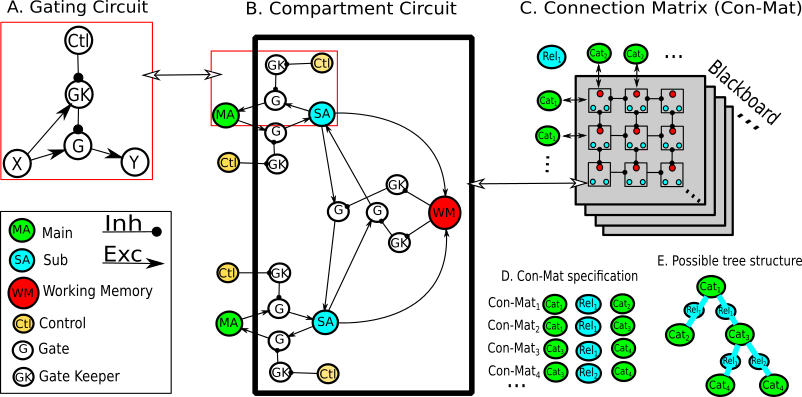
\includegraphics[width=1.00\columnwidth]{figures/gating_circuit3/gating_circuit3}
\caption{{\label{Blackboard} Blackboard architecture.
A. Gating circuit that allows the implementation of conditional neural
activity transfer between Neural assemblies X and Y through a gate
assembly. The gate keeper assembly initially is also activated by the X
assembly and then inhibits the gate assembly, so a control assembly has
to inhibit the gate keeper assembly to let information flow through the
gate assembly. B. Architecture of one compartment circuit of a
connection matrix is shown. Six gating circuits are arranged such that
conditional bidirectional neural activity flow is possible between two
main assemblies. Control assemblies regulate the direction of
information flow and allow the activation of sub assemblies. The two sub
assemblies excite the working memory assembly which once activated
encode the binding of the main assemblies and allow activation to flow
between them if the controls allow it too. C. Each connection matrix
contain n by m compartment circuits that encode the same relationship
type between the same pair of assembly categories. There are m available
assemblies for one category and n available assemblies for the
complementary category and only one cell circuit can activate its
working memory assembly to link two particular assemblies due to mutual
row and column inhibition of cells in the connection matrix. The size of
the connection matrix effectively represents memory limitations. A
blackboard is composed of an arbitrary number of connection matrices
that encode different relationship types for a pair of assembly
categories. D. A blackboard is composed of multiple connection matrices,
where each of them is defined by two node categories and a relationship
type between them. E. Example of one possible tree structures out of the
infinite that can be represented based on the specified connection
matrices.%
}}
\end{center}
\end{figure}

An important feature of the blackboard architecture is its flexibility
to process and implicitly represent arbitrary tree structures. Most of
the previous blackboard simulations considered flat tree structures
corresponding to dependency grammars\cite{nivre2005dependency}, where as
expected the word grammatical categories elicit activity in MAs while
their dependencies are represented by activity in WM and SAs. This
overlooks other grammar theories that depend on constituency like a
phrase structure grammar\cite{gazdar1982phrase}, where it is also necessary
to instantiate MAs for phrasal categories. Nonetheless this can be
easily resolved by allowing a WM, activated by the binding of two word
categories, to instantiate activity in another MA, which can participate
in further bindings reflecting hierarchical structure.

Here we implement only the necessary parts of the NBA to model the
neural activity related to variable binding, which itself is enough to
instantiate the representation of an arbitrary sentence syntactic
structure if we take the grammar theory and parsing scheme as given.
This means that we simplify two important aspects of the circuit. The
first is that we will provide the signals of control directly to the
compartment circuits. Previous attempts to train the control
mechanism\cite{van_der_Velde_2010} were tailored only to specific grammatical
cases and creating a general control mechanism to test the neural
activity patterns would require a more varied dataset in grammatical
categories and would comprise computational linguistic efforts out of
the scope of this work. The second is that we do not model the dynamic
inhibition of competing blackboard compartment circuits, since this
would require hypothesis about the size of the blackboard, which would
be related to memory limitations and the total number of possible
grammatical categories to link in binary trees, which again would
require out of scope computational linguistic efforts. Moreover the
simplest selection mechanism behind competing blackboard compartment
circuits can be hypothesized to be uniformly random on available
compartments. This means that we are only testing the temporal patterns
of neural activity linked to a variable binding event in the case of two
words association. While in the case of complete sentences we are
testing predictions based on the average neural activity time series of
a collection of compartment circuits instantiated as demanded by the
given grammar theory and parsing scheme. These time series should allow
us to differentiate neural activity from different syntactic tree
morphologies and sizes. In this work we will compare the predicted
signature of variable binding with ECoG recordings and the predicted
average neural time series of complete sentences with Bold-fMRI
activation patterns.

\section{Methods}

{\label{488128}}

\subsection{Implementation of the NBA}\label{implementation-of-the-nba}

\subsubsection{Simplified approach to the blackboard
architecture}\label{simplified-approach-to-the-blackboard-architecture}

The present implementation of the blackboard architecture respects its
abstract mechanisms but do not implement them completely. Here we do not
simulate complete connection matrices, the compartment circuits mutual
inhibition mechanism is an operation for which there is no obvious
unique implementation. There is already a proof of concept to understand
the implementation of the mechanism in randomly connected networks,
nonetheless it does not yet achieve a complete circuit level
specification integrated with a complete blackboard architecture
\cite{van_der_Velde_2011}. Instead we just instantiate compartment circuits as
necessary, since in essence they would be selected randomly in a
connection matrix from available compartments in the hypothesized
blackboard.

The compartment circuit abstraction is enough to achieve our current
simulation goals, since the same mechanism is used in different
connection matrices and they might only differ in their memory capacity.
So we can consider the same compartment circuit simulation for all
different pairs of grammatical categories, where the circuits would have
similar dynamics and only vary in activation time of their neural
populations. Nonetheless we are only able to ignore the activity of
complete connection matrices because we are not planning to explore the
effect of memory limits under time compressed sentence processing
scenarios or memory tasks. Otherwise important deviations in background
neural activity due to depletion of available compartments in the
connection matrices and intense inhibitory activity would become a
crucial factor in the simulation. This could be an interesting
exploration in future work to try to reproduce the temporal bottleneck
effects on neural activity shown by Vagharchakian et al. under
conditions of compressed speech and reading\cite{Vagharchakian_2012}.

In the case of the control mechanism, Feed-forward artificial neural
networks have already been employed with the NBA \cite{van_der_Velde_2010} and
recently state of the art feedforward network architectures have shown
top performance for diverse language parsing tasks \cite{Andor_2016}.
Moreover a more recent extension of the NBA relying on the motor circuit
of the marine mollusk Tritonia diomedea to generate patterns for
sequential activation control has been proposed\cite{van_Dijk_2015}.
Nonetheless implementing these neural architectures would be out of the
scope of this work, since we will not investigate the whole neural
activity related to parsing but only the portion specifically related
with variable binding, which itself is enough to look into the formation
and storage of a phrase structure with temporal events derived from some
some given parsing mechanism. Where also the expected phrase structure
is given by some specified grammar theory. So we will simply provide the
control signals that will allow the necessary neural activity flow from
MAs to WM to process the hypothesized syntactic structure as required by
a given parsing scheme and grammar theory.

\subsubsection{Simulation framework and architectural
decisions}\label{simulation-framework-and-architectural-decisions}

Previous simulations of the blackboard approximate the mean activity of
neural assemblies with Wilson Cowan dynamics \cite{Frank_2014}.
Nonetheless direct simulations of leaky-integrate-and-fire (LIF) neurons
\cite{omurtag2000simulation} have faster transient behavior than the pseudo
dynamics described by the Wilson Cowan equations. Such equations, as
explained by De Kamps \cite{de_Kamps_2008}, only allow to approximate
correctly the steady state of neural populations by suggesting what mean
firing rates should be. On the other hand, population density techniques
\cite{de2013generic} implemented in the MIIND software \cite{de_Kamps_2008}
\cite{harrison2011new} can accurately describe the transient dynamics of
large populations of the mentioned LIF neurons.

In Figure \ref{pdt_case} one can see an important difference between the
transient dynamics of the rate-based Wilson Cowan dynamics and the
population density techniques. Moreover one can appreciate how well
population density techniques approximate the precise simulation of the
LIF point neuron model presented by Omurtag \cite{omurtag2000simulation}. In this
work we are interested in modelling the transient dynamics of variable
binding with the future aim of comparing the simulation with real
temporally detailed patterns of neural measurements like ECoG. So we
opted to implement the compartment circuits with population density
techniques in MIIND instead of Wilson Cowan dynamics.

One could further argue that it is desirable to implement even more
realistic simulations approximating conductance based neural models and
neuron point models as those implementable with the RON, GENESIS and
NEST software reviewed by Brette et al. \cite{brette2007simulation}. Nonetheless
it has been shown that simpler 2D models like adaptive exponential
integrate-and-fire (AdEx) can already predict correctly 96\% of the
spikes of detailed conductance models\cite{brette2005adaptive}. Although the
model has the strong simplification of only considering one adaptation
time constant, when in reality adaption takes palce on multiple time
scales, it reproduces many known electrophysiological features, as can
be appreciated in the spike-frequency adaptation review of Benda et
al.\cite{Benda_2003,Benda_2014}. AdEx can also be approximated with population
density techniques and has been recently added to MIIND. Although it is
at least two orders of magnitude more computationally expensive than a
LIF model, it is feasible to implement it in a circuit with tens of
populations like the one we will simulate. So we will implement the
circuit under a LIF and an AdEx model to show the effects of adaptation
in the neural dynamics of variable binding under the NBA framework. To
our knowledge this is the first time that the AdEx model will be
employed to approximate the neural dynamics of a circuit of this
magnitude reproducing cognitive function.

In the case of Delay Activity (DA) populations like WM, we decided as a
first approach to model such mechanism artificially. We plan to address
the different alternatives to model persistent cortical activity with
interacting neural populations in future work. As suggested by De
Kamps\cite{de_Kamps_2005} not only models of recurrent excitation but
also recurrent inhibition can account for this phenomena. In the current
simulation a constant firing rate is kicked off by a specified level of
input that is sustained for a desired period of time. Contrary to
previous simulations \cite{velde2015ambiguity}, we do not consider SAs as DA
populations. We find that SAs can show rich and interesting dynamics
just by fulfilling their function of mediating activation for WM. In the
case of MAs we model them as receiving input from WM populations instead
of considering them as another DA population. This is done mostly to
separate the notion of a concept stored in a WM from the recruitment of
the MAs during parsing that would need to take place during sentence
processing. Moreover this allow us to easily instantiate deep tree
hierarchical structures by considering the WM of one circuit as the
source of activity that drives the MA of the next compartment circuit in
the hierarchy. The details of this implementation will become clear in
following sections.

\begin{figure}[h!]
\begin{center}
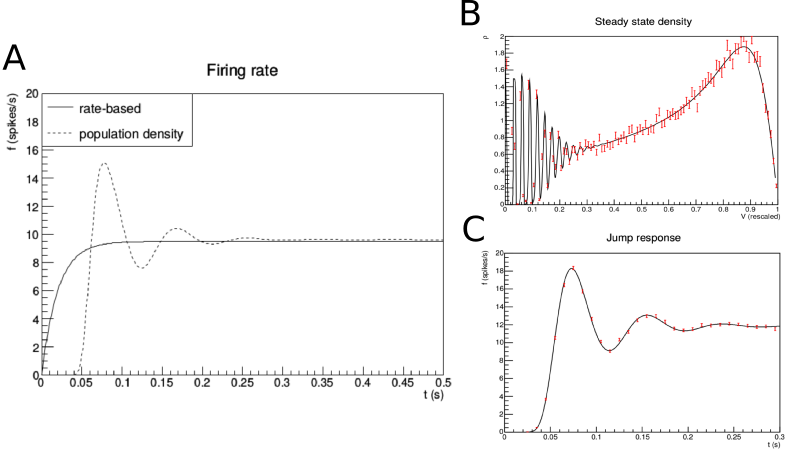
\includegraphics[width=0.70\columnwidth]{figures/case_for_pdt1/case_for_pdt1}
\caption{{\label{pdt_case} Case for population density techniques over Wilson
Cowan dynamics.
Plots taken from the MIIND manual. A. Shows the mean firing rate of a
neural population simulated with Wilson Cowan dynamics, labeled as a
rate based model, and a population density technique with similar mean
and standard deviation of neural activity. One can see that the steady
state of the population activity converge in time but that the transient
dynamics are importantly different. B. Histogram of the membrane
potential for each neuron in the population density technique simulation
shown in A at time 0.3. The solid line corresponds to the prediction of
the population density technique, while the red markers correspond to
error bars due to finite sample sizes in a point model simulation
performed with NEST. C. The jump response of the neural population
according to the NEST simulation and the population density technique.
There is complete agreement within the boundaries of statistical error.%
}}
\end{center}
\end{figure}

\subsubsection{Compartment circuit
parameters}\label{compartment-circuit-parameters}

The compartment circuit contains two different types of neural
populations. Artificial neural populations following a boxcar event
model and biological neural populations following LIF or AdEx neural
models. Both biological neural models have a wide range of parameters
that have been tuned in the literature to follow the behavior of a
regular spiking pyramidal cell in the cortex according to
electro-physiological measurements. These were taken from Omurtag et al.
(2000) \cite{omurtag2000simulation} in the case of LIF neurons and from Brette et
al. (2005) \cite{Brette_2005} in the case of AdEx neurons. As a first
step we wanted to only explore the behavior of the circuit of neural
populations in generality following well studied sets of parameters.
Nonetheless it is clear that studying the neural dynamics of specific
brain regions might require adapting the parameters of the neural models
to local measurements. Also considering parallely multiple neuron
typologies and modelling their corresponding microcircuitry of cortical
columns as attempted already with LIF models to simulate local field
potentials for a very small patch of cortex\cite{Mazzoni_2015,Hagen_2015}. Each
neural population can be either excitatory or inhibitory and so only
connections from the same type can come from them, respecting Dale's
law. The biological neural populations are conformed by a pair of Main
Assemblies (MA), a pair of Sub Assemblies (SA), six Gate Assemblies (G)
and six Gate Keeper Assemblies (GK). On the other hand the artificial
neural populations are conformed by Control assemblies (Ctl), Working
memory assemblies (WM), Event Input Assemblies (Inp) and a Baseline
Assembly (B) that drives baseline neural activity. A complete diagram of
the compartment circuit with example parameter values for LIF
populations is given in Figure 3.

That the artificial populations follow a boxcar event model means that
we just have to specify the starting point of events, the persistent
firing rate of the population and the duration of the persistent
activity. In the case of the delay activity of WM we also have to
provide a kickoff input rate threshold that automatically triggers the
boxcar event instead of providing a start time point. The duration of
persistent activity was pragmatically set up long enough to visualize
the steady state of the neural dynamics. Finally the persistent activity
rate and kickoff rate threshold were arbitrarily selected from feasible
parameter range values given by various simulations of the circuit
dynamics that will become clear in the following section.

Selecting firing rates to tune the compartment circuit is a complex task
given the contrast between the extremely simplified circuit and real
neural networks that contain multiple types of neurons with diverging
behavior across cortical layers \cite{Wohrer_2013}. Wohrer et al
\cite{Wohrer_2013} shows, from measurements in rat cortex, that the
actual firing rate distributions of neural networks do not differ much
between resting state and evoked activity. The small difference would
come from very few neurons that manage to drive up the mean firing rate
in recordings while most neurons in the population are almost silent,
some with rates as low as 0.1 Hz \cite{Kerr_2005}, whose activity
might not even be picked up by most recording devices. Although
theoretical analysis of the distribution of firing rates in randomly
recurrently connected networks of LIF neurons near the
fluctuation-driven regime suggests considering mean firing rates around
6.4 Hz \cite{Roxin_2011}. Based on the review of Wohrer et al.
\cite{Wohrer_2013}, particularly on the firing rate in motor areas of
behaving macaques, we decided to kickstart biological neural populations
activity up to a conservative baseline firing rate of 1 Hz and study the
neural dynamics of circuit input firing rates of up to 10Hz.

There are two parameters governing transmission of neural activity
between neural populations. First we consider the synaptic efficacy of
connections, which was setup to be homogeneous across the circuit under
the lack of appropriate hypothesis to tinker it in a detailed manner. As
exposed by London \cite{London_2002}, current understanding of synapsis
is limited and even contextual measurements of efficacy might be more
appropriate to understand the impact of synaptic input on spike output
that actual set parameters of the synapse. Moreover recent evidence
\cite{Briggs_2013} shows that synaptic efficacy might be modulated by
attention processes and is naive to consider it as a fixed parameter in
a circuit. The study of Briggs \cite{Briggs_2013} suggest that
synchronous firing of neurons with the same input has probabilities
between 3.1 and 7.6 while single firing has probabilities ranging from
28\% to 36\% depending on the type of neurons considered and the
attention state. Based on these reports, we decided to verify, through
an initial sub-circuit experiment, the effect that synaptic efficacy
could have on the circuit temporal dynamics, contrasting a low (10\%)
and high (30\%) value of synaptic efficacy for both LIF and AdEx
populations. This allowed us to verify if the tradeoff between efficacy
and number of connections was a trivial one, simply requiring more
connections when assuming a lower efficacy to attain similar ouput
firing rates for the same input rates. This, as will be shown in the
results section, was not the case for AdEx populations. Nonetheless the
difference in the qualitative nature of the temporal dynamics was
confirmed to not be crucial for the circuit setup, so for the remaining
simulations we employed the more conservative 10\% synaptic efficacy
regime.

The second parameter governing transmission of neural activity was the
number of connections between a pair of neural populations. Unlike
synaptic efficacy, the number of connections were determined from a
series of simulation experiments. First the number of connections from
baseline persistent activity was set such that, during rest, the circuit
steady state activity would stabilize around 1 Hz. The number of
baseline connections necessary is a function of input firing rate,
synaptic efficacy and neural model, such that a lower synaptic efficacy
required a higher number of connections. Then the number of connections
coming from excitatory populations was determined such that
bidirectional gating circuits would have a stable steady state firing
rate when both Gs allow neural activity to be transmited. Finally the
number of connections coming from inhibitory nodes were setup high
enough to block neural activity flow in a gating circuit, which means
that GKs driven by MAs would be able to completely inhibit activity in
Gs. Our simple approach to neural rate transmission ignores many
intricacies like activity regimes that might allow rich internal
computations. \cite{Ostojic_2014}. Also connections distribution might
have an impact in spike based communication \cite{Teramae_2012}. Still
we decided to keep connections between populations as simple and
homogeneous as possible for a first approach.

\begin{figure}[h!]
\begin{center}
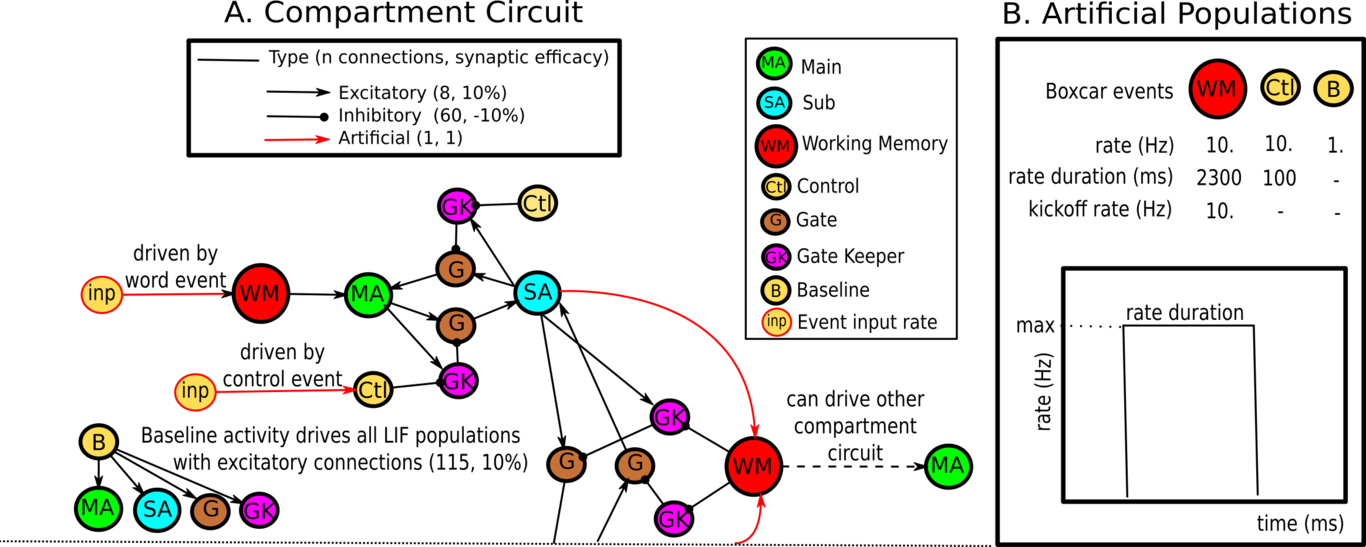
\includegraphics[width=1.00\columnwidth]{figures/circuit_specs3/circuit_specs3}
\caption{{Compartment circuit example
{\label{471683}}
A. Details of the Compartment Circuit implementation. Only half of the
circuit is shown since the design is symmetric. The baseline (B) and
Event input (Inp) populations are part of the simulation and not of the
original abstract circuit proposal. B. The behavior of the artificial
neural populations and their selected parameters is shown%
}}
\end{center}
\end{figure}

\subsubsection{Simulation experiments
performed}\label{simulation-experiments-performed}

Since it is possible to tune the circuit to reproduce arbitrary firing
rate values under which circuit dynamics are similar and stable, we
simply aimed at picking reasonable parameter values such that the
circuit would mantain overall modest firing rate values with respect to
the literature of neural measurements. To setup parameters and compare
in detail the compartment circuit dynamics for LIF and AdEx neural
populations, four simulation experiments were performed taking different
sub-circuits into account. A diagram of each sub-circuit is shown in
Figure 4. The first simulation simply consists on the activity of one
neural population driven by a fix activity rate of 1 Hz. We used this
simulation to explore the necessary number of baseline connections to
drive baseline activity in the circuit to approximately 1 Hz. The second
simulation allowed us to explore how neural activity flows through a
chain of neural populations being regulated by a control mechanism. The
third simulation explores how neural activity is enhanced by a closed
loop between a MA and SA, since it will be the case in the memory
sub-circuit that activity is allowed to flow bidirectionally once the WM
delay activity is unleashed. Finally the fourth simulation consists on
adding GKs to the closed loop sub-circuit of the second simulation to
explore how many inhibitory connections are necessary to keep activity
from flowing in the circuit unless the controls allow it.

After determining reasonable parameter values, we simulated the complete
circuit, portrayed in Figure 3, for both LIF and AdEX neural
populations. Then we contrasted the obtained neural patterns of the MA,
SA, G and GK neural populations with binding and constituency effects
available in the neuroimaging literature. First we show similitudes
between the activity of one compartment circuit and ECoG time series
patterns of binding revealed by Nelson et al\cite{Nelson_2017}. We
naively compare the firing rates of our simulation directly to the
patterns observed in ECoG recordings, considering the correlation that
exist between the high gamma power of local field potential signals and
firing rates\cite{Ray_2011,Manning_2009}. Nonetheless a quantitative comparison
would require a more careful consideration, employing recent models
tuned to electro-physiological measurements that offer a way to
translate neural activity to local field potentials\cite{Mazzoni_2015,Hagen_2015}.

Then we simulate the binding activity related to the processing of
complete phrases. Assuming a syntactic tree structure given by a phrase
grammar theory and the order of control events given by a bottom up
parsing scheme. As a first simplified approximation to the NBA dynamics,
we instantiated parallely the necessary compartment circuits to
represent a complete assumed tree structure. Once we obtained time
series for the processing of the entire phrase, by summing activity
across similar node categories of the multiple compartment circuits
required, we convolved the time series with the Glover Hemodynamic
Response Function\cite{Glover_1999}. This allowed us to approximate the
hemodynamic constituency effects depicted by Pallier et al.
(2011)\cite{Pallier_2011}. We managed to show that the sublinear function
that surprised the authors, governing the amplitude of HRF responses for
the different stimuli categories, is approximated by the dynamics of
binding events assumed by the NBA.

Since the quantitative level of neural activity can be easily tuned for
a wide range of parameter values with similar behavior, when comparing
the circuit neural dynamics with the neuroimaging literature, we only
focused on the qualitative neural temporal patterns observed. All the
C++ scripts behind the circuit and sub-circuit simulations, taking
advantage of the MIIND software\cite{de_Kamps_2008}\cite{harrison2011new}, are
accessible in the Blackboard application folder of the MIIND github
repository https://github.com/dekamps/miind.

\begin{figure}[h!]
\begin{center}
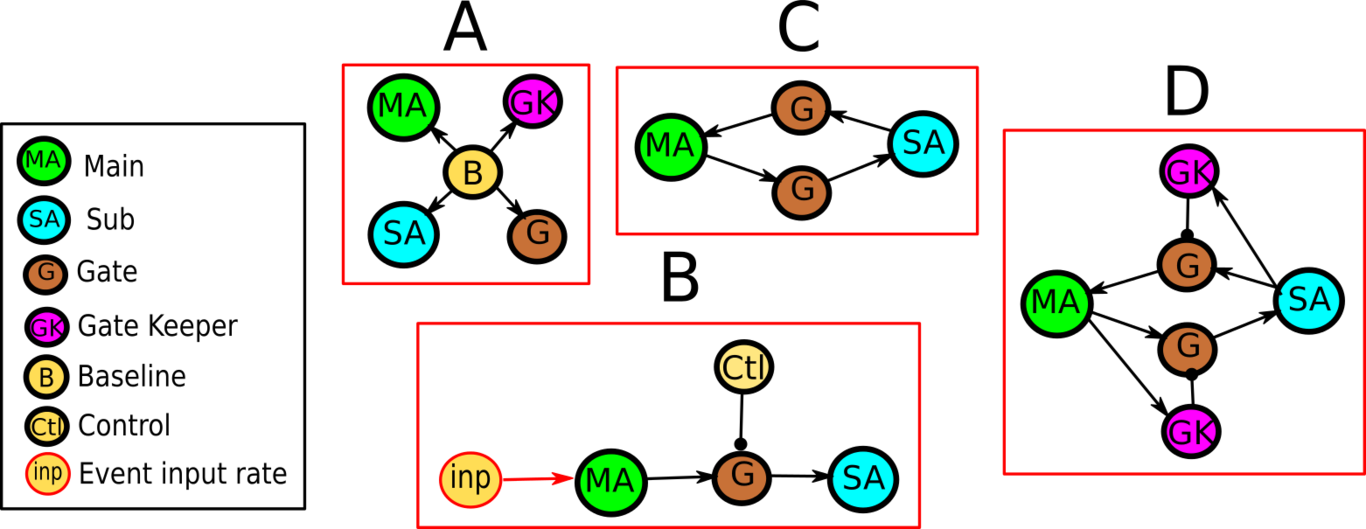
\includegraphics[width=0.70\columnwidth]{figures/sub_circuits3/sub_circuits3}
\caption{{Sub-circuit simulation topologies
{\label{637398}}
Each number corresponds to its respective experiment. For better
visualization all baseline nodes are excluded from the topologies. A.
Single neural population driven by baseline activity. This topology~
reminds of the fact that all MA, SA, G and GK populations are driven
initially in the same way by a persistent baseline fixed rate. B. Chain
of populations where activity is temporally interrupted by a control
node. C. Closed loop formed by MA, SA and Gs. D. Closed loop broken by
the addition of GKs.
{\label{637398}}%
}}
\end{center}
\end{figure}

\section{Results}

{\label{765620}}

\subsection{Sub-circuit simulations}

{\label{152250}}

\subsubsection{Experiment 1: Simple neural
population}

{\label{461536}}

The first experiment allowed us to explore the basic temporal behavior
of the different neural models under different synaptic efficacy
regimes. It also allowed us to select an appropriate number of baseline
connections to tune the steady state firing rate of all LIF and AdEx
neural populations to approximately 1Hz while being driven by a
persistent artificial 1Hz baseline rate. As indicated in the topology A
of Figure 4, all neural populations are driven identically by a baseline
node, so simulating one allow us to get an idea of the behavior of all
biological populations in isolation from the circuit connections.

As depicted in Figure 5, the steady state firing rate of LIF populations
is a monotonous increasing function of number of connections for both
synaptic efficacy values. We can see from the detailed temporal activity
that the firing rate increases gracefully until achieving the steady
state after approximately 200ms. On the other hand, the AdEx populations
behavior is qualitatively affected by the synaptic efficacy value
chosen. For a 10\% efficacy the steady state behaves like a monotonous
increasing function as in the case of LIF populations but for a 30\%
efficacy we observe a concave behavior due to extreme adaptation that
limits the steady state rate to a maximum below 1Hz. If we look at the
temporal details, the Adex populations also behave differently from LIF
populations. They portray a sudden increase of activity on initial
stimulation that is then driven down by adaptation, achieving a steady
state after approximately 600ms.

Based on these observations we decided to consider only the low efficacy
regime of 10\% for the remaining simulations. In the case of LIF
populations the higher efficacy would not bring any qualitative
modification to the dynamics of the circuit. In the case of the AdEx
population the only important qualitative difference would be
constraining the use of the steady state rate of activity, which would
itself force a tighter coordination of events. This more strict event
coordination can also be understood from the more permissive low
efficacy regime as will become clear in the following simulations and
discussion. Finally we learned that the number of baseline connections
that best approximate a 1Hz steady state firing rate are 115 and 1646,
for LIF and AdEx populations respectively, which will be fixed for all
remaining simulations.

\begin{figure}[h!]
\begin{center}
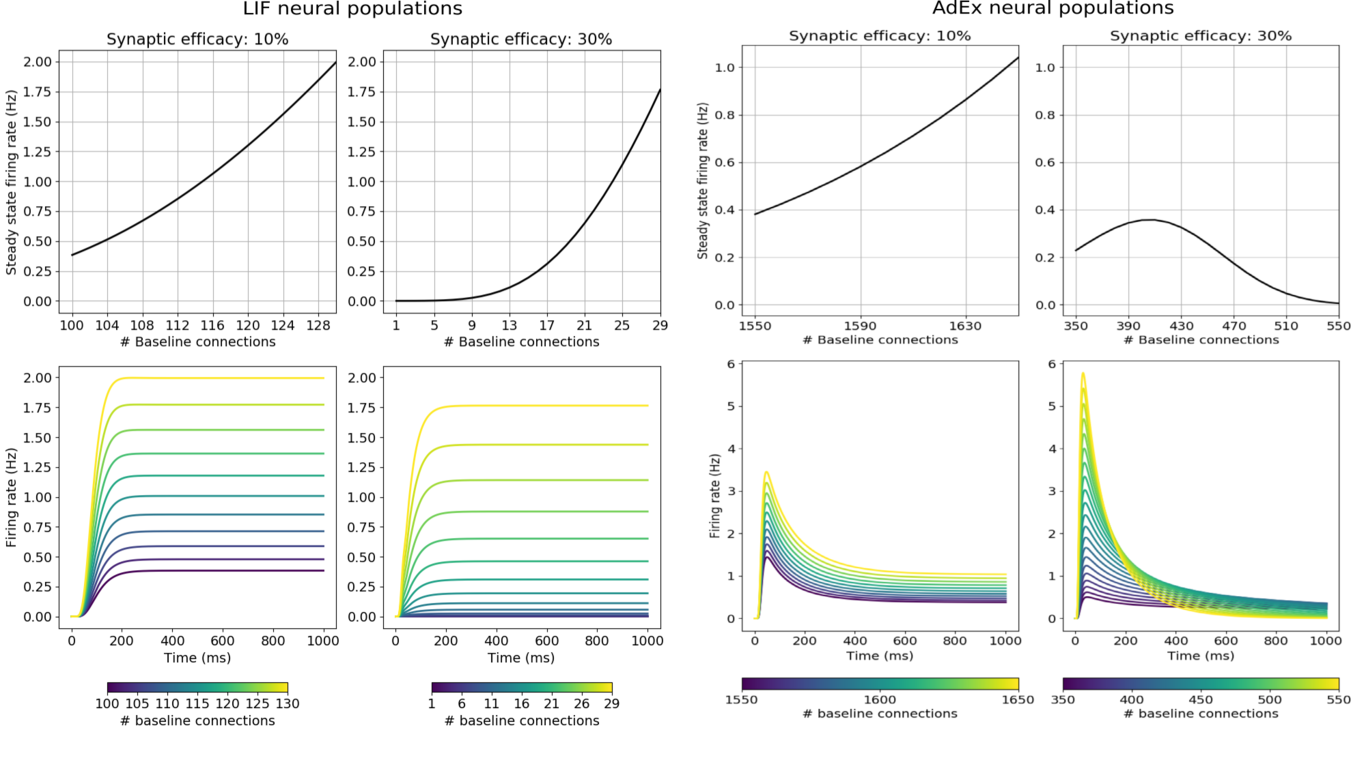
\includegraphics[width=1.00\columnwidth]{figures/experiment_001/experiment_001}
\caption{Baseline neural dynamics
The plots at the top depict how the steady state rate of a neural
population relates to the number of baseline connections under a
baseline input of 1Hz. The plots at the bottom show example temporal
dynamics corresponding to its upper plot.}
\label{674368}

\end{center}
\end{figure}

\subsubsection{Experiment 2: Neural activity flow and control
release}\label{experiment-2-neural-activity-flow-and-control-release}

In the second experiment we explored how the coordination of input and
control events would affect the rate of activity across a chain of
neural populations. We employed the topology B of Figure 4, in which a
fix input rate drives the activity of the sub-circuit during a given
time window and is mediated by a control operating under another time
window. This corresponds to a MA that attempts to drive up the activity
of G and SA, while a Ctl node inhibits the activity in G and isolates SA
activity from the input stimulation. The input and control events can
start at any arbitrary moment for any duration and what interests us are
the dynamics of the circuit when inhibition, assumed in the complete
circuit to be always present, stops allowing MA to freely excite G and
SA. There are three extreme cases that characterize the circuit
behavior. When the input starts and the circuit achieves the steady
state before G inhibition stops (Input first), when G inhibition stops
and the circuit achieves a steady state before the input starts (Control
first) and when both input starts and inhibition stops at the same
moment (Coordinated). Analyzing this sub-circuit let us determine what
kind of input rates are necessary to drive the maximum and steady state
rate of SA to some desired activation threshold for WM. Moreover it gave
insight into what are the most constrained type of events for each
neural model.

In Figure 6 we portray the neural dynamics of the last population of the
chain (SA). The steady state in a LIF model is achieved at a similar
time (under 200 ms) for all event cases. The Input first and Coordinated
events have a similar quantitative behavior, which means that the
dynamics of stopping inhibition are insensitive to MA having achieved a
steady state from the input stimulation. Nonetheless starting the input
on the absence of inhibition permits higher initial fluctuations of the
firing rate and so higher maximum rates of activity. On the other hand,
the AdEx model shows a more complicated behavior. Due to adaptation
effects, the maximum output rate response will depend on the current
state of the population. Basically~the closer the population is to its
steady state, the less responsive it will be due to the accumulated
adaptation. In AdEx populations the steady state takes longer to be
achieved (just approximated after 400ms) and its convergence rate
depends on the input rate and events combination. Also the maximum
firing rate of the dynamics strongly depends on the event case. Contrary
to the LIF model, stopping inhibition in advance minimizes the rate
dynamics due to the stronger adaptation present at the steady state of
G. Then starting the input before stopping inhibition improves the rate
dynamics at G and SA, which increase the further MA is from achieving a
steady state after the input starts and so are maximized with perfect
coordination of input and control.

From these observations we learn that the combination of events that
reduce the most the rate dynamics depend strongly on the neural model
selected. Being the Input first or Coordinated cases for the LIF model
and the Control first case for the AdEx model. Moreover, as is apparent
in Figure 6, the AdEx model requires a higher input rate to achieve
modest increases in the steady state of the output rate, which limits
the behavior of a circuit of AdEx populations under constant input
rates.

\begin{figure}[h!]
\begin{center}
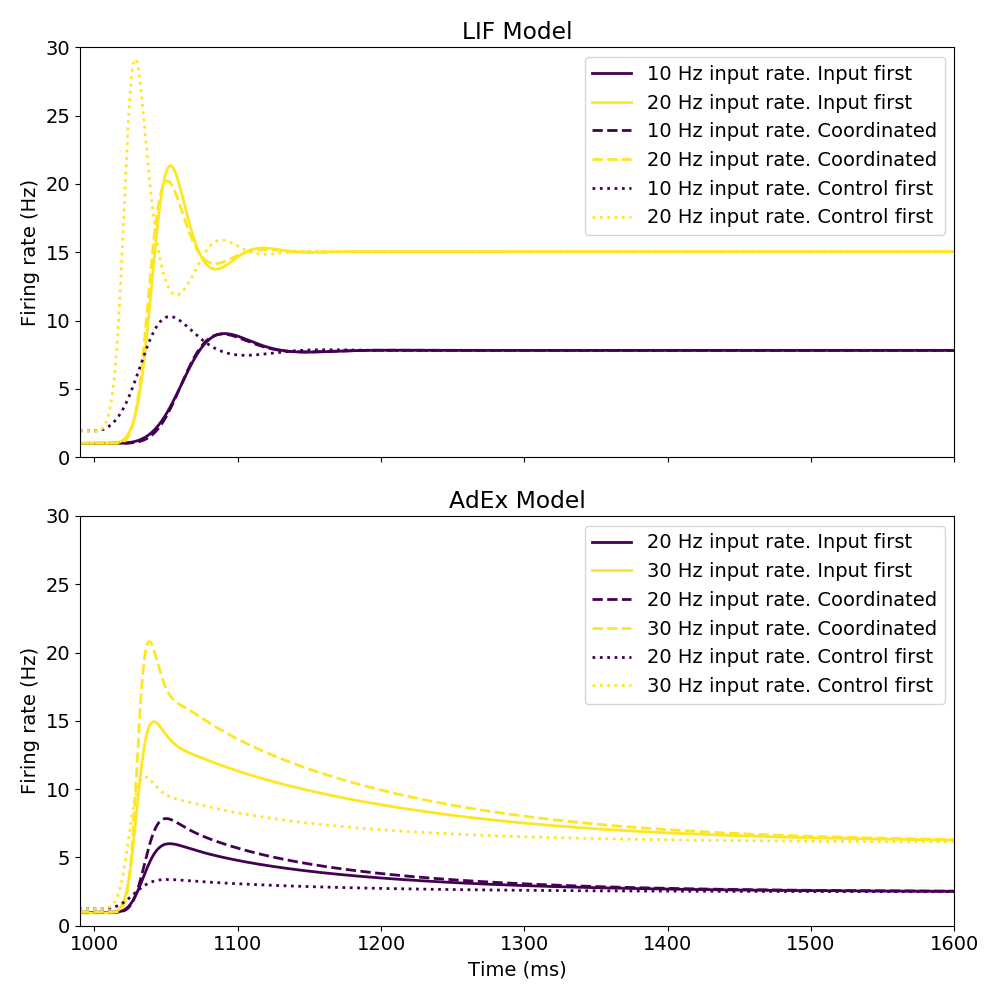
\includegraphics[width=0.70\columnwidth]{figures/experiment2_ctl_plots/experiment2_ctl_plots}
\caption{{Neural dynamics of input and control events
{\label{462003}}
For each neural model two input rates are simulated with the three
extreme combination of events: Input first, Control first and
Coordinated. ~9 and 20 excitatory connections are assumed for the LIF
and AdEx models respectively. We show the time series of the firing rate
in the last population of the chain (corresponding to a SA node of
topology B in Figure 4).
{\label{462003}}%
}}
\end{center}
\end{figure}

\subsubsection{Experiment 3:~Enhanced neural activity from closed
loop}

{\label{758539}}

In a third experiment we tested the behavior of the sub-circuit
corresponding to topology C of Figure 4. As was mentioned before there
is a number of excitatory connections after which the output rate is
higher than the input rate, such that populations wired in a closed loop
would enter an uncontrolled self reinforced activity regime. Since we
expect such a loop to exist in our circuit during activation of WM, we
had to constraint the number of excitatory connections employed. Another
important implication of the closed loop is that we would expect the
steady state activity of the populations to be higher than in their
independent states, which also gives a lower bound to the activation
threshold that we can select for WM, since otherwise WM would enter a
state of perpetual self activation after being activated the first time.
The steady state rate of the closed loop is shown in Figure 7 up to the
number of excitatory connections that would lead to an uncontrolled
activity regime.

Taking also into consideration the results of the second experiment we
can depict valid combinations of input rate, number of excitatory
connections and WM activation threshold. In figure 7 we show the steady
state rate (SS) curve for the events combination with the lowest rate
dynamics and the maximum rate (Max) curve for the events combination
with the highest rate dynamics. Notice that, as explained in the
previous experiment, the relevant combination of events in the analysis
are different in the case of LIF and AdEx populations. These curves
delimit four parameter regions with different implications for the
behavior of the NBA's memory circuit. The regions refer to the ranges of
values that the WM activation threshold can take according to a given
input rate and number of excitatory connections. The example curves
shown in Figure 7 correspond to an input of 10Hz and 25Hz for LIF and
AdEx populations respectively.

The perpetual activation region refers to the area below the steady
state of the closed loop activity and is independent of input rate. All
other regions depend on the input rate that determines the lowest and
highest rate dynamics. The flexible activation region refers to the area
between the closed loop curve and the steady state of the event
combination with the lowest rate dynamics. An activation threshold in
that region would secure activation of WM to any combination of events,
which makes it the most desirable range for the activation threshold.
The constrained activation region is bounded by the max temporal rate of
the highest rate dynamics and represent the range of values for which
the timing of input and control events is constrained. Finally the
impossible activation region is above the highest rate dynamics and
represent rate values that can not be reached by the circuit dynamics.

Characterizing the activation threshold regions is important to
understand the reliability of the circuit when exposed to noisy input
rates, arbitrary coordination of events, control mistakes or
anticipatory control signals. With precise control of input rates and
the timing of events corresponding to bottom up parsing, one could
simply select an activation threshold just above the minimum rate
dynamics to secure activation from the activity of two SAs. Nonetheless
there are other scenarios that we should be able to test with parsing
schemes diverging from pure bottom-up parsing, if we interpret
prediction as anticipated control activation. In that case, if
prediction fails we would be confronted with a control mistake for which
we would not want the circuit to perform a binding. This would be
illustrated by an input that drives activity in the first MA of a
compartment circuit followed by a control event that allows activity to
flow from all MAs, while the second MA never receives the input
corresponding to the activation of its concept. In such a case one would
need the threshold to be higher than the minimum of the impossible
activation region for a given input rate and number of excitatory
connections, such that the input of one SA alone could not trigger WM.
This additional constraint can itself push the activation threshold
beyond twice the maximum of the flexible activation region, forcing
coordination of at least one input and control event, as can be
appreciated for AdEx populations in Figure 7. To allow anticipatory
control mistakes for the complete circuit simulation we selected a
combination of 10Hz and 20Hz input rates, 8 and 20 excitatory
connections and 10Hz and 9Hz activation thresholds for LIF and AdEx
populations respectively.

\begin{figure}[h!]
\begin{center}
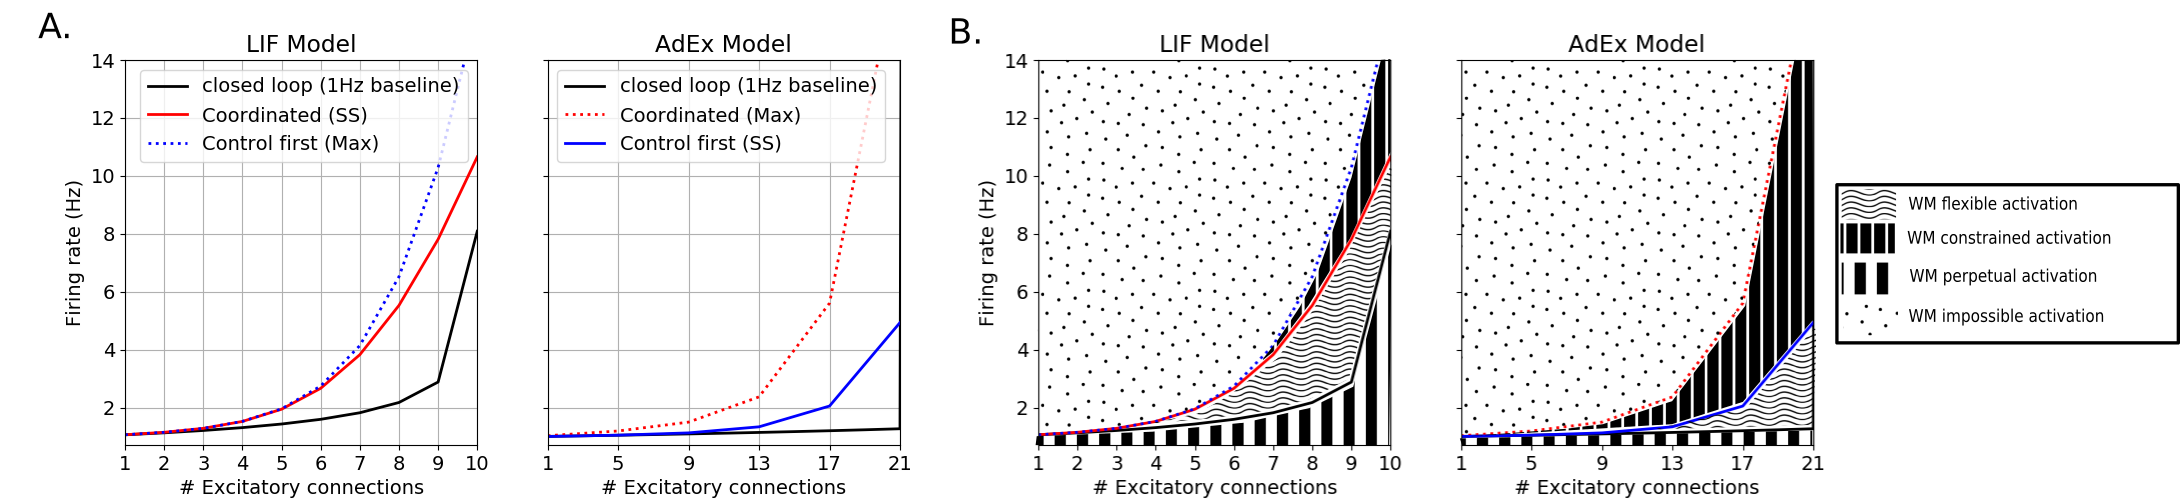
\includegraphics[width=0.70\columnwidth]{figures/experiment_3/experiment_3}
\caption{{Closed loop activity and memory sub-circuit activation regions
{\label{197355}}
Plots at the top show an example steady state and max activity rate of
the event combination with weaker rate dynamics, in contrast to the
steady state rate of the closed loop enhanced activity formed by WM
activation. Plots at the bottom identify the parameter regions, where
the WM steady state rate (SSR) and maximum rate (MR) threshold region is
the one that gives most constrained range of circuit parameters to offer
the most flexible coordination of input and control events. The event
rate curves correspond to an input rate of 10Hz and 25Hz for the LIF and
AdEx models respectively.~
{\label{197355}}%
}}
\end{center}
\end{figure}

\subsubsection{Experiment 4: Inhibition of closed loop enhanced neural
activity}

{\label{554287}}

For the fourth and last sub-circuit experiment, corresponding to
topology D of Figure 4. We aimed at tuning the amount of inhibitory
connections in the circuit such that the neural activity in GKs could
inhibit the activity in Gs when there is no intervention of control
signals. In this way we break permanently the closed loop of activity
unless a bidirectional control signal or WM activation allows it in the
complete circuit dynamics. To realize this we picked the number of
inhibitory connections necessary to inhibit max firing rates for the
wide range of number of excitatory connections allowed by the closed
loop dynamics. The maximum firing rate is employed instead of the steady
state rate to observe inhibition of the strongest fluctuations. Based on
the curves shown in Figure 8,~we set the number of inhibitory
connections to 70 and 250 for LIF and ADEX populations respectively for
the following simulations.



\begin{figure}[h!]
\begin{center}
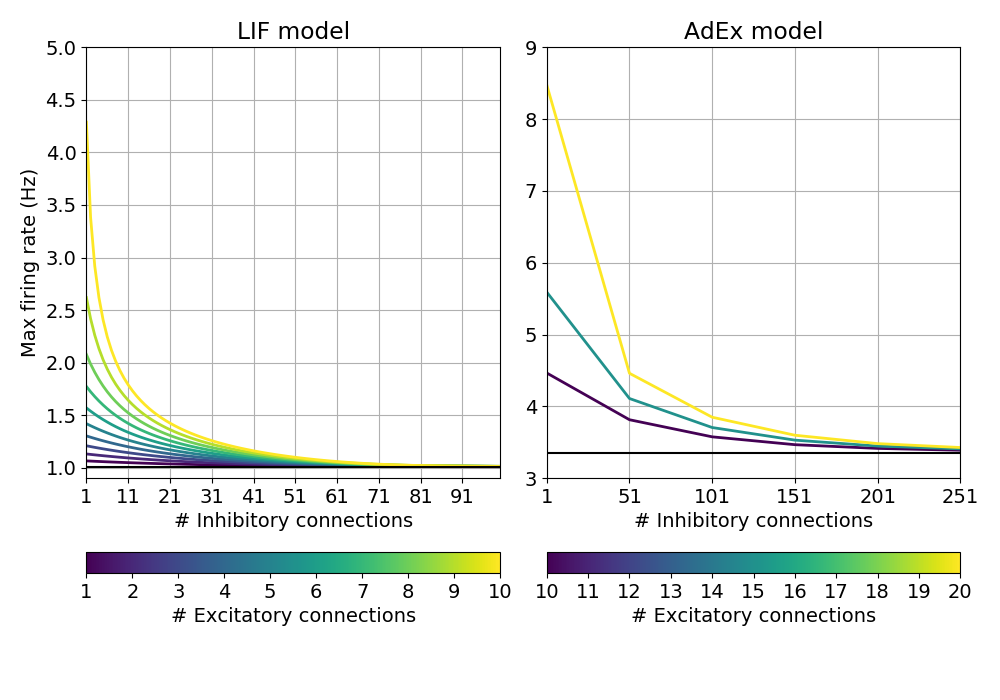
\includegraphics[width=0.70\columnwidth]{figures/experiment_4/experiment_4}
\caption{{Inhibition of closed loop neural activity
{\label{970310}}
Each curve represents how the maximum enhanced neural activity of ~a
closed loop circuit with a given number of excitatory connections is
driven back to baseline as we increase the number of inhibitory
connections. Considering a baseline rate approximating a 1 Hz steady
state in both Models. The maximum firing rate is employed instead of the
steady state rate to observe inhibition of the strongest fluctuations.
{\label{970310}}%
}}
\end{center}
\end{figure}

\subsection{Complete compartment circuit
simulations}

{\label{444332}}

After selecting a valid set of parameters from the observations of the
sub-circuit experiments we explored the behavior of the complete
compartment circuit simulation. The dynamics of the compartment circuit
can be summarized by a combination of the input events that drive
activity in MAs and the control events that inhibit GKs such that
activity can flow from MAs to Gs and SAs. In Table 1 we present a
summary of the parameters for LIF and AdEx simulations and in Figure 9
we present the temporal dynamics of the compartment circuit under
different combination of events.

\begin{table}[h!]
\centering
\normalsize\begin{tabular}{1.0\textwidth}{ CCC}
Parameter & LIF & AdEx \\
baseline connections & 115 & 1646 \\
excitatory connections & 8 & 20 \\
inhibitory connections & 70 & 250 \\
Baseline rate (Hz) & 10 & 20 \\
WM/Ctl rate (Hz) & 10 & 20 \\
\end{tabular}
\caption{{Complete simulation parameters
{\label{917316}}%
}}
\end{table}First we observed the dynamics of the circuit when no events take place,
leading to baseline activity. In this state all biological populations
are just receiving an input baseline rate of 1 Hz from the artificial
baseline neural population. Nonetheless instead of having an output rate
approximating 1 Hz as they would have in isolation, the different nodes
reflect with their firing rate the architecture of the circuit. Gs show
a low rate of activation due to GKs inhibition, while GKs how the
highest rate driven by MA and baseline activity. MAs show an activation
close to the approximated 1Hz baseline as well as SAs that have been
isolated in the circuit thanks to GKs inhibition. SAs have a slightly
higher steady state rate than MAs since they are the center recipient of
neural activity of the circuit and at least some neural activation
manages to leak the Gs. The baseline activity of the different neural
models can be seen in part A of figure 9.

Then in part B of Figure 9 we portray the partial activity of the
circuit. This means that only one MA receives a fix input rate and a Ctl
event takes place opening activity flow from both MAs to SAs.~We can
observe that, as expected, the increased activity of the stimulated MA
causes strong inhibitory activity in the GK that compensate the flow of
neural activity from MA to G to avoid activation of the corresponding
SA. Moreover it can be seen in Figure 9 that in the case that Ctl
activation takes place when only one MA is active, the circuit
effectively do not activate the binding WM and will simply return to an
appropriate steady state once Ctl stops.

Finally in part C of Figure 9 we can appreciate that in case both MAs
are active and a Ctl event takes place, then the binding will take place
by activation of WM.~During the process of binding the reverberating
activity of WM that inhibits the GKs connecting SAs creates a sudden
burst of activity leading to a pronounced spike as SAs become part of a
self excitatory closed loop, also elevating the activity of Gs and GKs
between them. This burst of activity quickly drops back to a steady
state that leaves the inner circuit in a higher level of activity with
respect to its original resting state, facilitating communication
between MAs. A similar behavior during sentence parsing was observed in
previous simulations of the NBA\cite{Frank_2014}.

Although the general qualitative behavior of the compartment circuit
architecture is similar for LIF and AdEx populations, there are three
important quantitative differences present but not easy to appreciate in
Figure 9. The first is that LIF population dynamics take longer to
transmit rates of activity since its transient oscillations are more
modest in proportion to the input rate. In these simulations, with the
same timing of events, WM became active 86 ms after all input and
control events take place in the LIF simulation, while in the AdEx
simulation this only took 42ms. The second is that the new enhanced
activity regime produced by WM activation is very sensitive to the
adaptation effect present in the AdEx model. Not only the parameters of
the neural model itself but also synaptic efficacy could completely
eliminate the higher sustained activity while keeping a high spike of
activity on the moment that binding takes place. The third is that the
AdEx simulation is sensitive also to small variations in the timing of
events due to the increasing influence of adaptation as populations
reach the steady state, while LIF model dynamics are only affected by
the input rate of the events.

\begin{figure}[h!]
\begin{center}
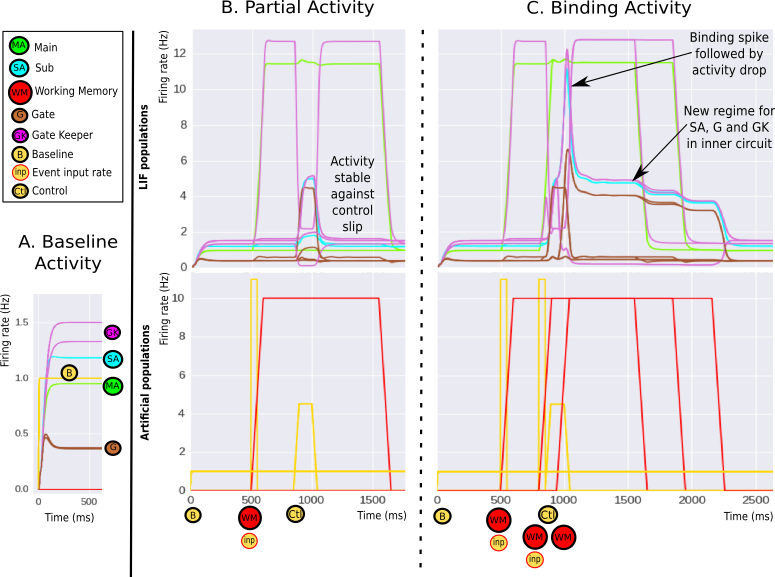
\includegraphics[width=0.70\columnwidth]{figures/activity_profiles/activity_profiles}
\caption{{\label{activity_profiles} Profiles of neural activity
A. Neural activation driven only by baseline input. B. Neural activation
of the circuit when only one MA is activated by a word event or WM at
500ms. Portrays the neural activity related to an erroneous control
signal at 850ms. Its possible to see that the steady state of neural
activity is resilient to a slip of control, going to the appropriate
levels of neural activity once the control activity is over. C. Neural
activity of the Compartment Circuit for a successful binding. The second
MA gets activated at 800ms followed by the controls at 850ms. Since both
MAs are active, the SAs manage to activate WM to instantiate the binding
of the MAs. Two interesting dynamics arise from the binding. The first
is that a spike of activity in SAs, GKs and Gs takes place due to the
sudden inhibitory activity of WM on the GKs. The second is that the
circuit internally raises its baseline activity.%
}}
\end{center}
\end{figure}

Once we have the neural dynamic of the compartment circuit, we can
extract key segments of transient activity and approximate the NBA
binding activity of complete phrases. For this approximation we can
consider parallely the necessary compartment circuits to build an
assumed underlying tree data structure given by a grammar theory. We
would also need a specification of the timing of parsing operations and
the desired duration of WM activity. The order of the parsing operations
can be taken from a bottom-up or more generalized left-corner parsing
scheme. Then the more precise timing of the parsing operations can be
assumed to depend on word presentation times for word bindings and
minimal operational constraints. Furthermore, we can think of the WM of
word bindings as the MAs of phrasal nodes and so on, which would then
give us the time at which a superior phrasal nodes input is available.

One can see in the example of Figure 10 how the hypothesized tree
structure of a sentence and the timing of the activation of tree nodes
is transformed into the neural activity of a blackboard. First we
substract the baseline activity profile from the binding activity
profile of the segments of neural dynamics used for the simulation. This
is motivated by our interest in making comparisons with neuroimaging
data. Then we simply add up the aligned time series of the different
compartment circuits by neural population category or some other desired
criteria. In the example, summaries of the activity of different neural
populations are shown as well as total activity of the blackboard
circuit assuming equal contribution from the different populations.
Certainly the way we should aggregate time series to compare them
quantitatively with neuroimaging data would depend on the spatial and
temporal resolution available and the assumptions made about the spatial
distribution of the blackboard architecture in the cortex. in the case
of WM activation it is reasonable to assume a duration at least long
enough to allow all bindings in the tree to take place at the rate that
words are presented to the blackboard. In this example words are
presented every 600 ms, so for illustrative purposes we assume WM is
active 2300ms to be able to bind the first word to an awaited phrase
node activated after presentation of the fourth word. If WM was active
for say less than 1900ms then activation of the first word MA would
cease before the accompanying phrasal node MA comes into play.

\begin{figure}[h!]
\begin{center}
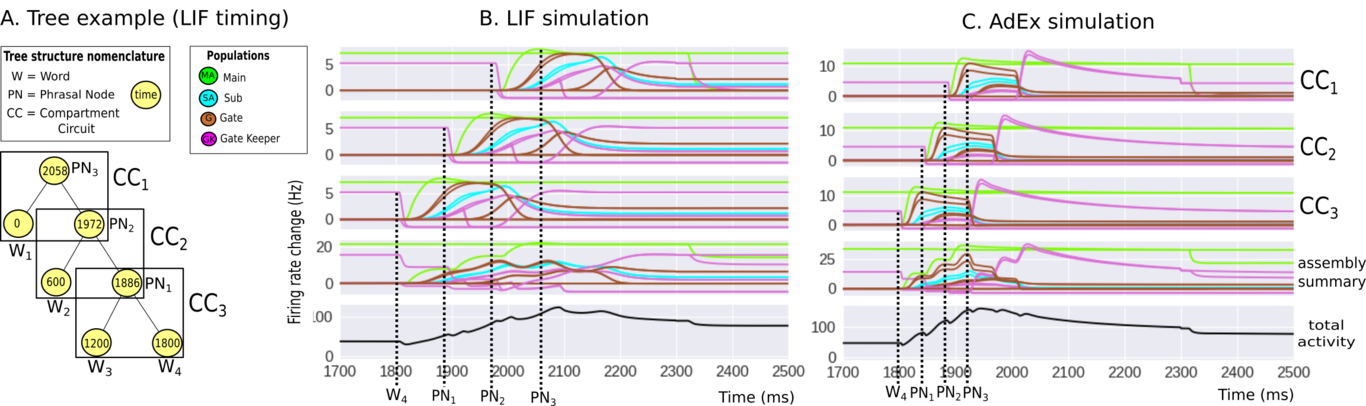
\includegraphics[width=1.00\columnwidth]{figures/compartments_tree_example/compartments_tree_example}
\caption{{Sentence processing example
{\label{679921}}
A. Tree structure hypothesized for a given 4 words phrase. It is shown
how compartment circuits correspond to sections of the tree structure
and how the nodes corresponding to grammatical categories of words
processed or phrase nodes are instantiated in time under a bottom-up
parsing approach. B. Blackboard time series that correspond to the
simulated processing of the considered tree structure and time of
activation of the nodes. The separate activity of the LIF populations of
each compartment circuit are shown separately, followed by their summary
and total activity C. Same as~B but for AdEx populations.
{\label{679921}}%
}}
\end{center}
\end{figure}

We can apply the complete phrase neural time series approximation to a
variety of stimuli from experimental designs behind neuroimaging results
in the literature. First we considered the simple case of increasing
size right branching trees that relate to a recent analysis of
intracortical (ECoG) recordings of a phrase reading
task\cite{Nelson_2017}. In this experimental design subjects had to keep
a phrase in memory to later compare it with a shorter probe phrase. We
make a qualitative comparison with caution, given that high gamma power
has been shown to be correlated to the firing rate time series of
spiking neurons from in-vivo recordings\cite{Ray_2011}.~In our
simulation, shown in Figure 11.A, we can appreciate four main temporal
segments of neural activity. An initial increase of activity dependent
on word presentation that reflects MA populations, a sudden rise and
drop of activity during WM activation, a decrease of activity paced by
the duration of input activity driving MA populations and a final drop
of activity when WM delay activity stops and the inner closed loop of
populations in the memory sub-circuit go back to its initial baseline
state. We also show, in Figure 11.B and 11.C., modified plots, extracted
from Nelson et al., reflecting the mean high gamma power time series of
the ECoG recordings.

As can be seen in Figure 11.B, there is an increase in baseline activity
when comparing the beginning and end of phrase processing that can be
interpreted as WM related activity based on the task. This memory effect
is reproduced in the NBA simulation by the enhanced activity of the
closed loop in the memory sub-circuit. It is represented by the
difference between the start of the simulation and the end of the MA
inactivation temporal segment, denoted in Figure 11 by black bars. It
could further be tuned to fit quantitatively the data by manipulating
the number of excitatory connections, such that their decrease would
reduce the baseline difference. The irregularities of the magnitude of
the baseline effect with respect to phrase length in the high gamma
power is difficult to interpret, since it could suggest that the
accumulation of activity with more recruiting nodes is subtler than what
we can reproduce with the NBA circuit, in which there is a clear
correspondence with the number of hypothesized compartment circuits of
the parsed tree structure. Moreover, when comparing simulations, we
appreciate that the AdEx model could better reflect a more modest
proportional increase of baseline thanks to adaptation.~

Another observation of the experiment is a proportionally important
~increase in activity during word processing. The peak magnitude and
onset of this increase seems to reflect the length of the phrase. This
effect can be captured by the simulation with a simple interpretation of
the accumulation of MA activity waiting to participate in bindings,
assuming a bottom-up parsing scheme. Nonetheless what was unexpected is
the spike of activity followed by a pronounced drop suggested naturally
by the NBA simulation, which is also emphasized by Nelson et al. in
Figure 11.C. This seems to be the case for both intermediate and final
bindings, with a drop magnitude dependent on the number of open nodes in
the assumed phrase grammar tree structure of the phrases. The number of
open nodes reflect accumulation of pending bindings under a bottom-up
parsing scheme in right branching sub-trees. The increasing drop
magnitude is captured in the simulation by the quick succession of
pending bindings in a tree structure. In the case of the LIF simulation,
there is flexibility to extend the activity peak with the duration of
control events and to increase the total drop magnitude by manipulating
the input rates and excitatory connections. On the other hand the AdEx
model loses this flexibility due to adaptation but better emphasizes the
contrast between the activity peak and sudden drop because of the
pronounced initial activity burst of its population dynamics.

There~is an issue with the interpretation of activity drops due to
binding operations. As can be seen in Figure 11.B, for the assumed right
branching phrase ``ten sad students of Bill Gates'', there is a sentence
middle drop that do not correspond to the prediction of a completely
bottom up parsing scheme. To accommodate this behavior into the NBA,
without changing our grammar and parsing assumptions, we would need to
incorporate a limited capacity to sustain MA activity that has to be
renovated or a greedy binding mechanism that leads to premature binding
mistakes. In the case of the sentence end, the final activity drop has a
steeper slope than the activity raise during sentence processing,
suggesting to incorporate a mechanism that releases MA activity after
binding takes place, which is unaccounted for in the simulation. Finally
in the analysis of Nelson et al. there is no depiction of WM
inactivation, likely due to the experimental design. Interestingly, the
AdEx simulation distinguishes itself from the LIF simulation, during WM
inactivation, by predicting a final burst of activity due to the
inhibition release of the GKs in the memory circuit. Nonetheless this
would be a difficult to appreciate marker in the oscillatory signal of
intracortical recordings.

\begin{figure}[h!]
\begin{center}
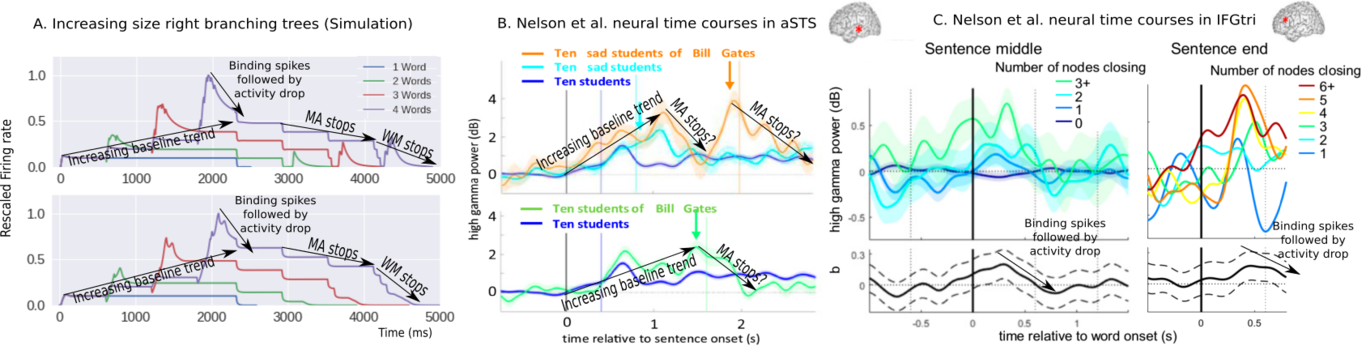
\includegraphics[width=1.00\columnwidth]{figures/ecog_comparison2/ecog_comparison2}
\caption{{Simulation comparison with intracortical (EcoG) recordings
{\label{286166}}%
}}
\end{center}
\end{figure}

We also considered the case of a more complex experimental design
employed to show constituency effects with Bold-fMRI\cite{Pallier_2011},
also based on right branching trees. In this experiment each stimuli
presented to a subject in a trial consisted of a list of phrases with
the same number of words (constituents), such that in total 12 words
would be presented. The conditions were one list of 12 unconnected words
(c01), 6 phrases of 2 words (c02), 4 phrases of 3 words (c03), 3 phrases
of 4 words (c04), 2 phrases of 6 words (c06) and 1 phrase of 12 words
(c12). This stimuli was simulated by repeating and adding the time
series of~each of the right branching trees in a condition. In figure 12
we contrast the NBA neural activity time series predicted by the LIF and
AdEx simulations for each condition with the simple Boxcar event model
used in experiments to estimate the amplitude of the hemodynamic
responses. We applied with a convolution operation, to each time series,
the Hemodynamic Response Function (HRF) proposed by
Glover\cite{Glover_1999}, taken from the python open source package
Nistats (\textbf{MISSING REFERENCE)}. This is a very naive approximation
taken for illustrative purposes, that has to be interpreted with caution
since the relationship between neural activity, cerebral blood flow and
blood oxygenation is not linear\cite{Friston_2000,Buxton_2004} and better represented
by the balloon model than the gamma function considered
here\cite{Waldorp_2009}.

In Figure 12 we mark the HRF peak and its onset with black lines on the
HRF convolved time series. It can be appreciated that the neural time
series would predict in all cases a peak onset displaced many seconds
with respect to the traditional boxcar event that only represents the
duration of the stimuli. Looking at the time series this would be
expected, since the HRF peak onset depends on the center of mass of the
accumulated response that continues several seconds after stimuli
presentation. Nonetheless a precise onset estimation depends on the MA
and WM inactivation periods that have been arbitrarily set in the
simulation to a constant, which leads to a superlinear increase of onset
based on number of constituents. This is unlikely from our previous
observations in ECoG recordings, that suggest a much faster decrease of
activity after stimuli presentation. Still this prediction gives a
cautionary tale on the extent to which lack of neural modelling can lead
to a non trivial misspecification of the events introduced in the GLM
model to analyze Bold-fMRI experiments. Thinking the other way around,
the peak onset link to the MA and WM inactivation periods suggest that
we could also use Bold-fMRI to fit the parameters of an inactivation
mechanism in the NBA. To realize this, such mechanism would need to be
proposed and a more realistic mapping from neural activity to blood
oxygenation would need to be implemented. As a last remark related to
HRF peak onset, one can appreciate that the LIF neural model introduces
an additional onset delay with respect to the AdEx neural model, due to
its slower activation of bindings.

\begin{figure}[h!]
\begin{center}
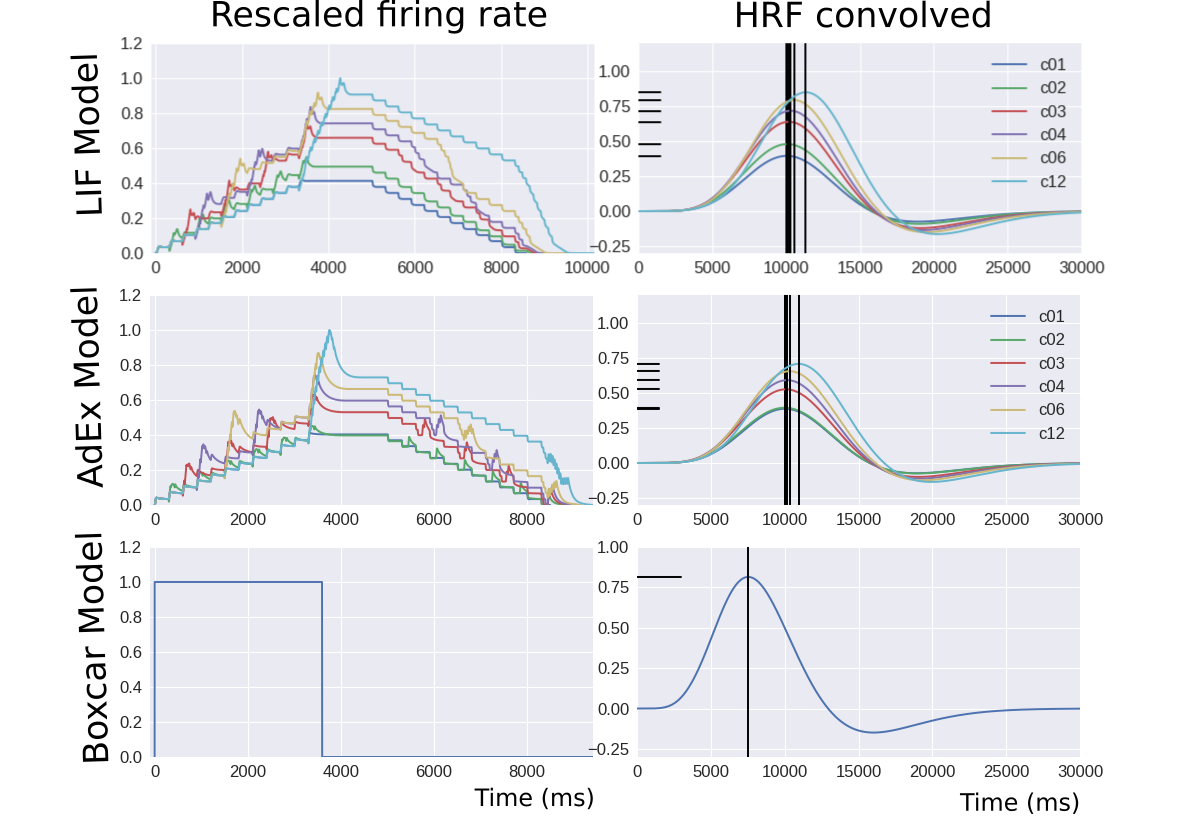
\includegraphics[width=1.00\columnwidth]{figures/pnas_comparison01/pnas_comparison01}
\caption{{Simulation hemodynamics interpretation
{\label{473368}}%
}}
\end{center}
\end{figure}

On the other hand, both AdEx and LIF simulations predict a similar
pattern on the increase of the amplitude of the HRF peak for conditions
with increasing constituent size. Since the peak depends mostly on the
number of nodes of the assumed tree structures, it is more interesting
to compare it qualitatively with the experiment. Our simulations
reproduce the sub-linear response that surprised initially the authors,
who were testing a linear hypothesis. In addition to normal phrases,
Pallier et al. designed a jabberwocky stimuli in which function words
are preserved and other words are replaced by morphological similar but
undefined words. While there are constituent responses in the language
areas TP, aSTS, pSTS, TPJ, IForb and IFtri, only the regions pSTS,
IFGorb and IFGtri portray a similar response pattern even when
minimizing the semantic content of phrases with jabberwocky. Since our
simulation puts aside semantic considerations, this type of experimental
manipulation is a better reflection of the activity linked to the
compartment circuit of the NBA, in contrast to the aSTS time series
previously analyzed on the ECoG dataset.

We portray in Figure 13 the simulations predicted pattern alongside the
ones revealed in pSTS, IFGorb and IFGtri language regions for the
jabberwocky stimuli.~The LIF and ADEX predictions are very similar,
except for the word list condition. Notice that the contrast of the
amplitude of word lists with the other conditions can give insights into
the relative proportion between MA and WM activity. As we saw in the
ECoG time series, MA seems to have a more important participation in the
total neural activity than we initially modeled. This could explain
the~flatter slope of the experimental results. To reproduce it with our
simulations, keeping their qualitative behavior intact, we could select
a parameter regime with less excitatory connections and higher input
rate. Note that in the case of the AdEx model, due to the shape of the
adaptive response, it would be possible to reproduce the sublinear peak
amplitude effect while minimizing a peak onset difference. To achieve
this we could make all responses approximate the same center of mass by
mixing the high initial increase of firing rate, that depend mostly on
the input rate, with a very low steady state rate. Nonetheless, to make
a quantitative fit to the hemodynamic amplitudes we should use a more
realistic hemodynamic model and be cautious about the possible model
misspecifications introduced by the simultaneous consideration of the
HRF peak onsets.

\begin{figure}[h!]
\begin{center}
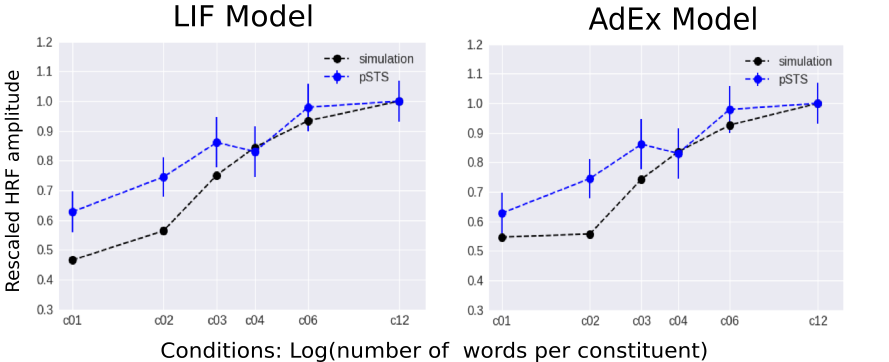
\includegraphics[width=1.00\columnwidth]{figures/pnas_comparison-02/pnas_comparison-02}
\caption{{Simulation comparison with Bold-fMRI experiment
{\label{395077}}%
}}
\end{center}
\end{figure}

\section{Discussion}

{\label{160055}}

An important insight from this work is the sensitivity of the neural
activity interpretation to the underlying neural model selected. Even in
the case of hemodynamic responses that average out circuit details, we
find trade-offs between the LIF and AdEx models. For example that an
AdEx model would offer more flexibility in our circuit to manipulate HRF
peak amplitudes while minimizing their onsets. To our knowledge this is
the first work to explore more complex models like AdEx alongside LIF
for variable binding and language function related circuits. There were
also many predictions of the NBA independent of the model selected, like
the fact that we need a high number of inhibitory connections and so of
inhibitory activity to avoid uncontrolled regimes of self excitatory
activity dependent on the connectivity of the circuit.

A more subtle exploration that was considered out of the scope of the
work would be to appropriately consider the cell parameters in the
models based on electrophysiological recordings from specific brain
regions, in contrast to the Omurtag~\cite{omurtag2000simulation}~Brette et al.
parameters~\cite{Brette_2005}. There are indeed different adaptation
constants along the cortex and we have compared the simulation
constantly with specific language related brain regions like aSTS, pSTS,
IFGtri and IFGorb.

In the case of the complete circuit assumptions, some of them were still
overly simplistic. We approximate baseline dynamics with a simple low
constant input rate instead of also considering the natural oscillatory
activity of the cortex, more appropriate homeostatic mechanisms in
cortical circuits\cite{turrigiano2011too} and balanced
networks\cite{Wolf_2014}. Setting up the synaptic distribution of the
network have important implications in terms of energy consumption,
while allowing random connectivity could importantly constrain control
of closed loop connections. This last consideration is interesting in
itself as a research question and could have an impact in the study of
the temporal bottlenecks observed in language
processing\cite{Vagharchakian_2012}. Introducing modular cytoarchitectonic
considerations on the populations that conform the circuit would allow a
better spatial interpretation of the circuit activity in a cortex patch
and might be anyway necessary to accurately translate firing rates into
Local Field Potentials\cite{Mazzoni_2015,Hagen_2015},
hemodynamics~\cite{Buxton_2004} and other promising measurement
techniques.

Moreover the nature of WM delay activity was left out of the current
work due to its flexible and still debated
implementation\cite{de_Kamps_2005}, but studying it could reveal important
neurobiological limitations on the way we asses the proportion of MA and
WM activity and the spatio-temporal memory limitations of the circuit. A
final missing consideration that has been partially tackled in previous
work\cite{van_der_Velde_2011} is how such a circuit architecture can be formed
during learning and brain development. We obviously do not expect the
hardwired architecture modeled here to represent the biological reality
but to facilitate an approximation to its behavior. Demonstrating how
mechanisms approximated by the architecture can actually be learned with
biological realistic Hebbian or STDP rules alongside random connectivity
constraints, during development, is an important avenue of future
research.

The simulation results show how both the steady state and transient
dynamics of the circuit affect our interpretation of the neuroimaging
evidence for language processing. In contrast to previous
simulations\cite{van_der_Velde_2011,van_der_Velde_2010,Frank_2014,van_Dijk_2015}, employing population density techniques
implemented in the MIIND software\cite{de_Kamps_2008,harrison2011new} allowed us to
approximate well transient temporal dynamics. Thanks to this, we could
show an important difference in the shape of the AdEx and LIF responses,
how before arriving to a steady state AdEx responds differently to
additional input due to adaptation and how the coordination of input and
control events is importantly influenced by the model and its
parameters. This last point is crucial for language processing, since
ideally~we would want input and control events to be as independent as
possible to diminish operational complexity and to be able to operate
under a wide range of parameters allowing for random variation.
Reflecting on the coordinating complications introduced by adaptation we
would expect lower adaptation in language related brain regions that
seem to be involved in binding operations like pSTS, IFGTri and IFGorb,
an increase in the operational complexity of the circuits and/or a
reduction in the operational parameter ranges alongside additional
sensitivity to noise. A final remark related to event coordination
problems in AdEx would be its sensitivity to the synaptic efficacy
parameter of the circuit that was not explored in detail. Contrary to
the LIF model, AdEx requires clear limitations in the populations
connectivity to implement arbitrary or complex timing operations.

An important aspect of this work, that could be overlooked, is the
flexibility of the simulation to represent the neural activity of many
grammar theories and parsing schemes. We can without circuit
modification implement any concept represented as a binary tree. This
corresponds well for example to the phrase grammar of the minimalist
program of Chomsky\cite{Chomsky_2014}~and to grammatical relations in
dependency grammars\cite{nivre2005dependency}. Nonetheless in the case of
dependency grammars we would not need to extend the memory of MA less
than in a phrase grammar that requires to wait for the instantiation of
phrase nodes in deep hierarchical trees. Also the AdEx model would favor
shallower tree representations, because it is sensitive to complex event
coordination.

Also so far we have implicitly considered activation of phrase nodes
only as a result of word binding, which would be representative of a
bottom-up parsing approach. This allowed us to simply take the binding
WM activity of one compartment circuit as the MA of another compartment
circuit. Nonetheless we did not introduce additional delays in control,
since we did not model the portion of the NBA responsible for control.
Naturally there are many additional parsing mechanisms that we could
assume, represented by the order of input and control events, that would
introduce predictive control activity. This would be the case if we
extend our analysis to the~generalized left corner parsing proposed by
Hale\cite{hale2014automaton}. We could interpret this additional predictive
control signals as control anticipation or as direct activation of
memory circuits that have to be deactivated later by an error signal.
Exploring the neural activity implications of both these mechanisms
alongside the target tree structures given by alternative grammar
theories is an important target of future research. This could be done
for example by using the simulation as an experiment design tool that
provides the set of phrases that maximize the spatio-temporal
differences in neural responses across conditions defined under the
different grammar theories and parsing schemes.

Finally, even though there are still many limitations in these
simulations, we would like to emphasize the quick progress in the
development of biologically plausible models of cognition. With an
additional effort it would be possible to fit parameters of the circuit
and phrase processing directly to neuroimaging measurements. Also
diverse new computational methods like population density techniques
have made it feasible to approximate at a circuit scale point neural
models as complex as the adaptive exponential. There are as well
successful recent efforts in modeling, with cytoarchitectonic details,
complex signals like Local Field Potentials~\cite{Mazzoni_2015,Hagen_2015} and
hemodynamics with the balloon model~\cite{Buxton_2004}. These could be
already adapted to our circuit simulations to better incorporate
neuroimaging evidence simultaneously from multiple techniques and
experimental designs. Moreover the circuit itself can become a tool for
hypothesis exploration and experimental design on the different
neuroimaging techniques. In conclusion we hope~to have shown that we are
close to producing biologically realistic mechanistic neural models of
cognitive function, that could provide new ways of testing cognitive
hypothesis on varied neuroimaging techniques, to further~inspire more
work in this direction.

\selectlanguage{english}
\bibliographystyle{plos2015}
\bibliography{bibliography/converted_to_latex.bib%
}

\end{document}

